% This Source Code Form is subject to the terms of the Mozilla Public
% License, v. 2.0. If a copy of the MPL was not distributed with this
% file, You can obtain one at http://mozilla.org/MPL/2.0/.
%
% Copyright (c) 2011-2019 ETH Zurich.

\begin{chapter}{Trace Partitioning in Sample}
	\label{chapter:Extension}

	This chapter presents my implementation of the trace partitioning abstract domain and its integration into \sample.\\

	Before discussing various implementation details, Section \ref{section:DomainRepresentation} illustrates how the concepts of the trace partitioning domain from Chapter \ref{chapter:TracePartitioning} are adapted to the concrete implementation. Section \ref{section:PartitionedState} then continues by presenting an alternative \code{State} implementation, the core of the extension. The necessary modifications to \sample to use this new \code{State} implementation are the subject of Section \ref{section:Integration}. The flexibility of the implementation is then demonstrated with the various directives in Section \ref{section:Directives} before Section \ref{section:UserInterface} presents the extension of an already existing user interface. Finally, Section \ref{section:Limitations} addresses some of the shortcomings of the current implementation and suggests some future extensions.

	% DOMAIN REPRESENTATION

	\begin{section}{Domain Representation}
		\label{section:DomainRepresentation}

		The main challenge of a trace partitioning implementation lies in representing the elements $(T, P^T, \Phi)$ of the trace partitioning domain. This implementation assumes that $\Phi$ is of the form $\Phi: (L \times T) \to D$ for some guest domain $D$. It can therefore be, by curryfication, represented in the form $\Phi: L \to (T \to D)$. This has the advantage that the static analysis can be performed as described in \ref{section:StaticAnalysis} using a states of the form $T \to D$. 

		% Tokens

		\begin{subsection}{Tokens}
			As Mauborgne and Rival suggest, tokens from $T$ represent decisions that have been taken during the analysis along the control flow. Since in the end it is desirable to have easy access to multiple decisions made during the analysis, the singleton tokens used so far are impractical. A more flexible approach is therefore needed.

			\begin{definition}[Token]
				A token in $T$ can be represented as a stack of labels from some label set $E$. A token is then either
				\begin{itemize}
					\item the initial token denoted by \emph{\code{init}},
					\item a label $e \in E$ or
					\item the combination of two tokens $t,t' \in T$ represented as $t::t'$.
				\end{itemize}
			\end{definition}

			The following example illustrates the use of tokens to keep track of decisions and how using a stack representation results in a more intuitive approach.

			\begin{example}[Tokens]
				Coming back to the extended system $P^{T'}$ from Example \ref{example:extendedsystem} with the token set $T' = \{t_0,\ t_1,\ t_2\}$, recall the interpretation of the tokens:
				\begin{itemize}
					\item $t_0$: The initial token, nothing has been decided.
					\item $t_1$: The analysis follows along the \code{true} branch of the conditional.
					\item $t_2$: The \code{false} branch has been chosen during the analysis.
				\end{itemize}
				Using the newly introduced notation, the elements can be reinterpreted starting with the initial token \code{init} instead of $t_0$. The two tokens discerning the two branches are then $\code{init}::\code{If(2,true)}$ and $\code{init}::\code{If(2,false)}$ respectively. The name of the label (\code{If}) indicates that a decision has been made about following a conditional. The first argument points to the location of the conditional in question and the second argument indicates which branch has been taken.

				Suppose the \code{true} branch contained another conditional where the distinction of the two branches benefits the analysis. The tokens generated for this distinction will then be the stacks $\code{init}::\code{If(2,true)}::\code{If(4,true)}$ and $\code{init}::\code{If(2,true)}::\code{If(4,false)}$.
				\exampleend
			\end{example}
		\end{subsection}

		% Directives

		\begin{subsection}{Directives}
			The tokens need to be generated during the analysis. The mechanism responsible for doing it is called a directive. A directive specifies the kind of distinctions it can make by providing a list of tokens representing possible choices. Applying such a directive to a token $t$ then leads to the tokens that result from pushing each token specified in the directive on top of $t$. A special case is the directive for merging partitions which, instead of appending tokens to a stack, removes them. The details of this operation will be discussed later.

			\begin{example}[Directive]
				The $\code{PartitionIf}$ directive that distinguishes between executions along the two branches of a conditional at position $i$ generates the two tokens $\code{If(i,true)}$ and $\code{If(i,false)}$ representing the two possible choices. Applying the directive to some token $t$ results in $t::\code{If(i,true)}$ and $t::\code{If(i,false)}$.
				\exampleend
			\end{example}

			These directives could be generated from annotations in the source code or, for example, from heuristics. This implementation requires them to be provided externally. The way to do this at the moment is either by means of writing analysis specific code or by using the user interface discussed later on.
		\end{subsection}
	\end{section}

	% ARCHITECTURE

	\begin{section}{Architecture}
		\label{section:PartitionedState}

		The core of the implementation is depicted in Figure \ref{figure:tracepartitioning}. At the center lies the class \code{PartitionedState}. The partitioned state represents the full state of the analysis at a given location. That is, at any point $l \in L$ during the analysis the state must keep track of the mapping from tokens to states of the guest domain ($T \to D$).

		\begin{figure}
			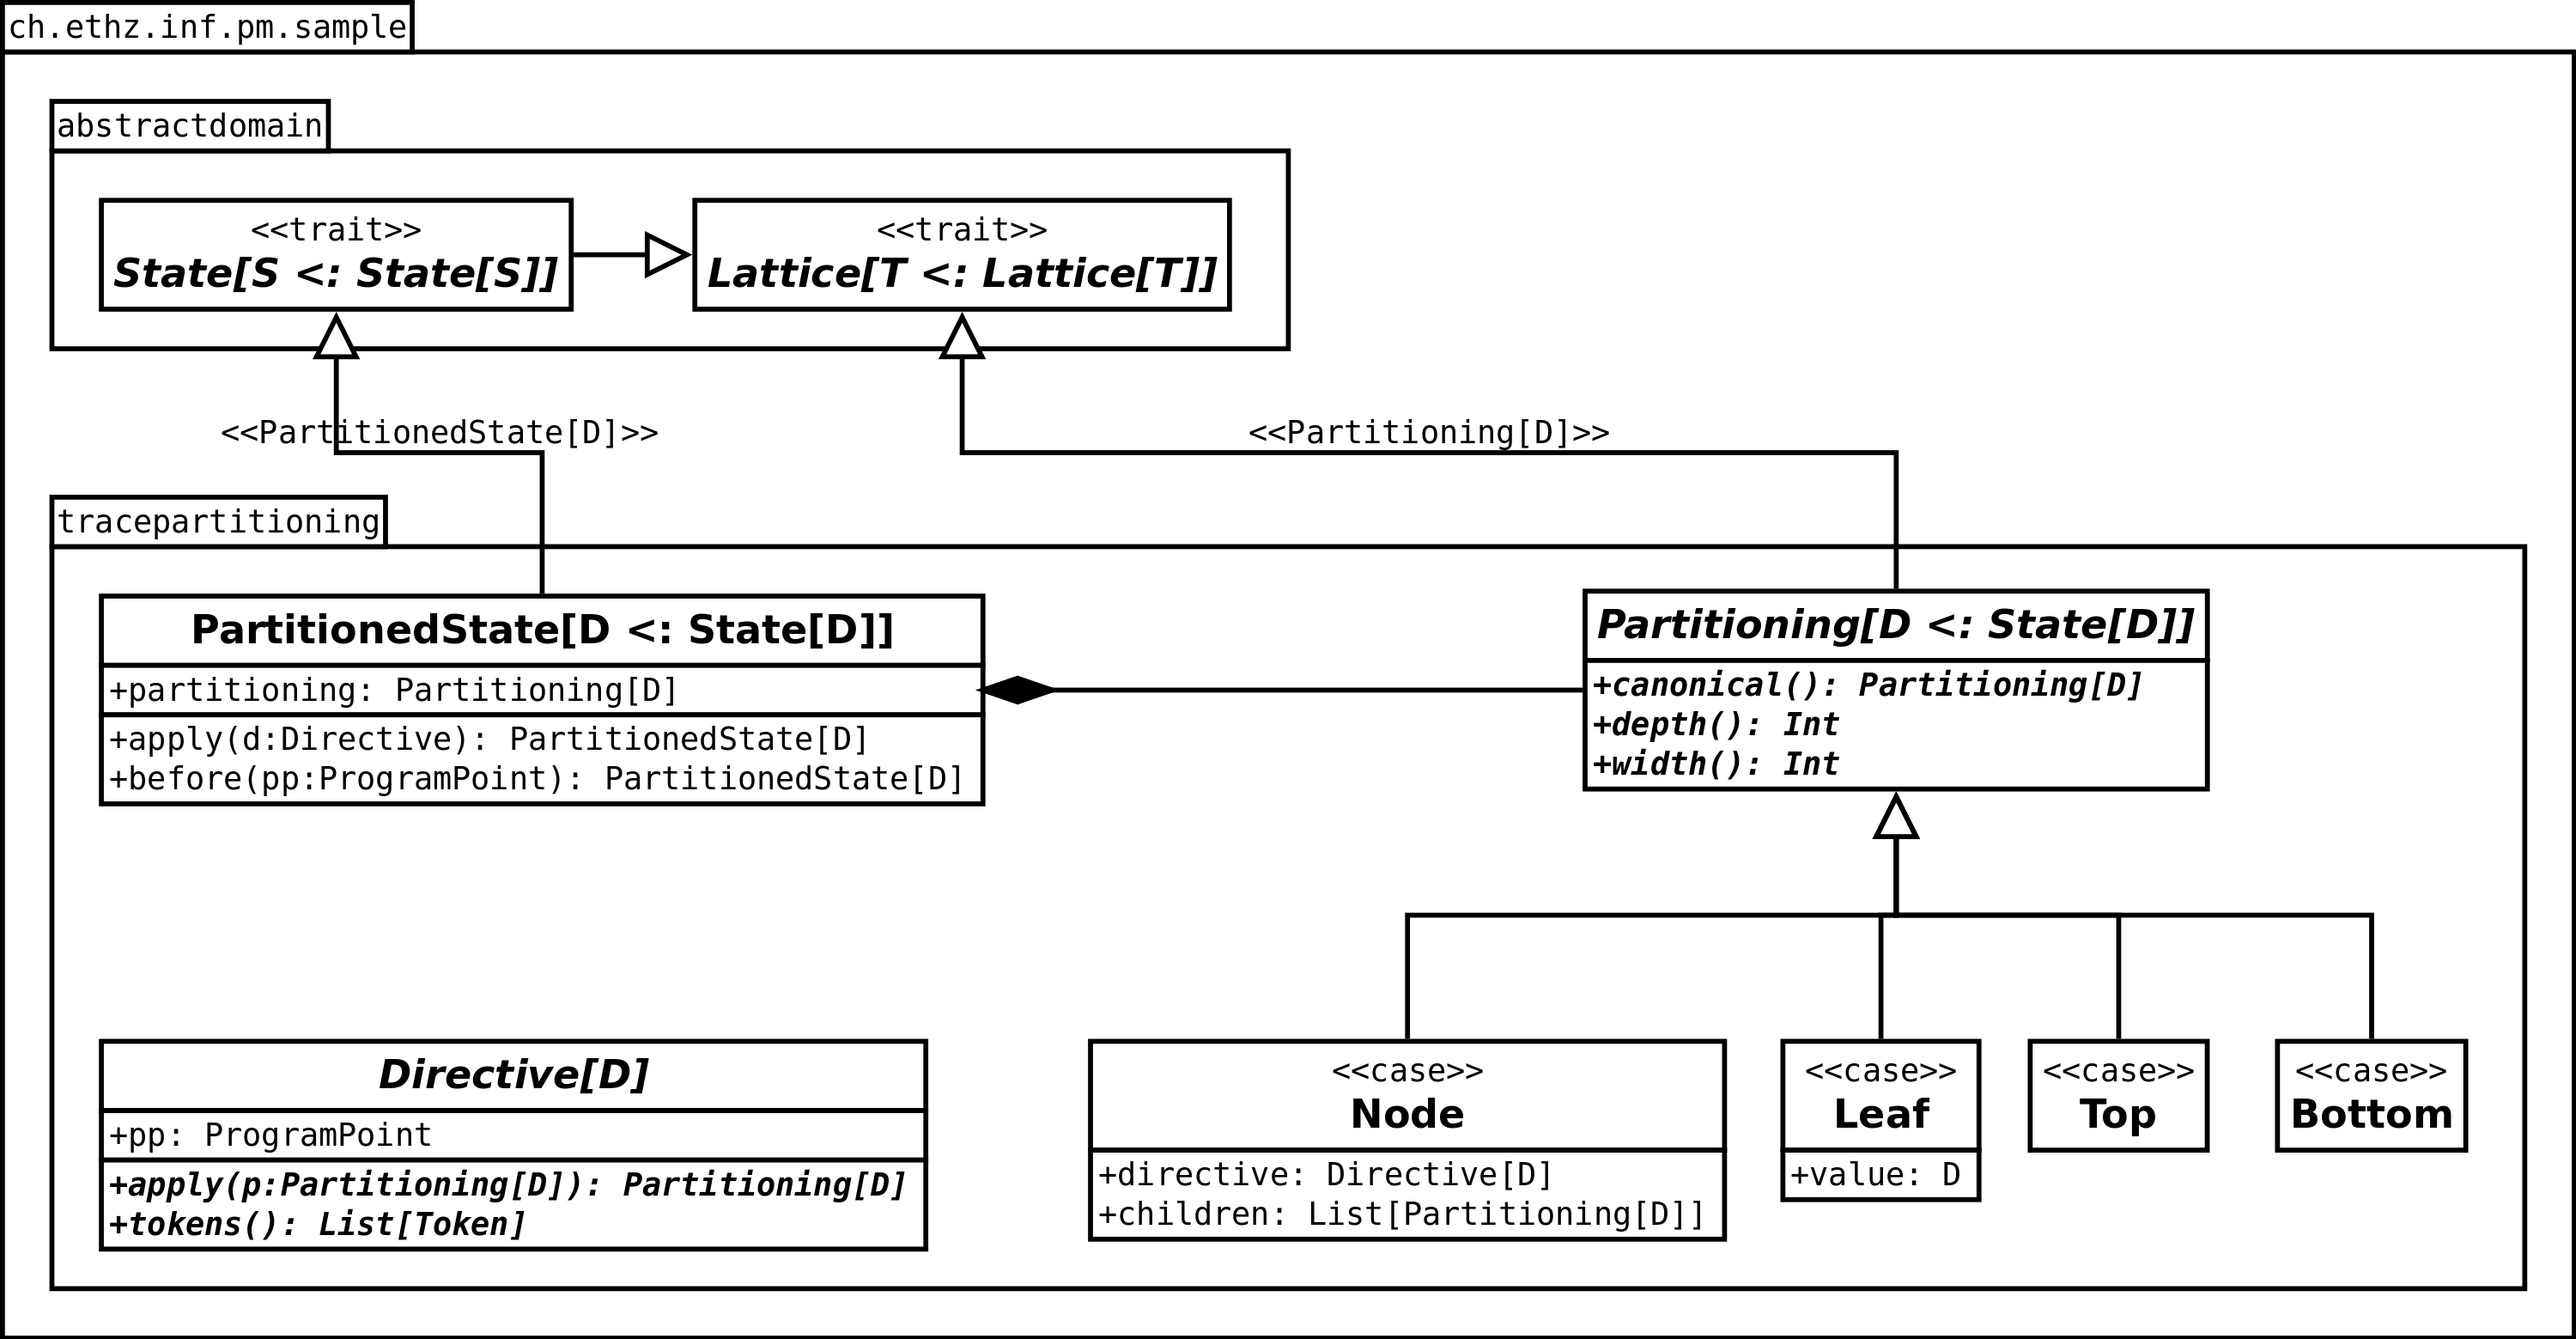
\includegraphics[width=\textwidth]{Diagrams/tracepartitioning.png}
			\caption{The \code{tracepartitioning} Package}
			\label{figure:tracepartitioning}
		\end{figure}

		This mapping can be efficiently represented by a tree structure where the nodes consist of the directives mapping tokens to their children. At the leaves of the tree are the states of the guest domain. This structure is implemented by the abstract class \code{Partitioning}. Each partitioned state consists of one such partitioning.

		As a general rule, the responsibilities of the two classes \code{PartitionedState} and \code{Partitioning} are split as follows. The partitioned state's main concern is the implementation of the \code{State} trait and providing interfaces for directives and for the analysis. The partitioning, on the other hand, solely manages the tree structure and is mainly concerned with the lattice operations.

		The directives are represented by the abstract \code{Directive} class. Implementing classes have to override the \code{apply} method that is responsible for transforming the tree structure. Furthermore, they have to provide a list of tokens they generate. Since directives are applied between statements, each directive is identified by the program point of the statement it precedes. More details and example implementations will be provided in Section \ref{section:Directives}. 

		% Partitioned State

		\begin{subsection}{Partitioned State}
			\label{subsection:PartitionedState}

			The \code{PartitionedState} is similar to the \code{GenericAbstractState} in that it provides some default implementation of the \code{State} trait. The type parameter \code{D} represents the kind of guest domain. This guest domain is typically a generic abstract state.

			% Semantic Operations

			\begin{subsubsection}{Semantic Operations}
				Implementing the \code{State} trait seems straightforward but comes with its own set of challenges. Apart from the \code{testTrue} and \code{testFalse} methods, which require feedback from some directives (cf. Section \ref{section:Directives}), the semantic operations (e.g. \code{createVariable}) are simply redirected to the leaves of the partitioning.

				The main challenge is introduced by the nondeterministic symbolic abstract values. Functions which do not contain abstract values in their arguments are mapped to the leaf states using the private helper function \code{map} that takes as argument a function transforming a leaf (\code{f: D => D}) and applies this function to all leaves of the partitioning. Listing \ref{listing:PartitionedState::createObject} illustrates the usage of the \code{map} function.

				\lstinputlisting[float=h, caption=The \code{createObject} Method, label=listing:PartitionedState::createObject]{Source/PartitionedState_createObject.scala}

				When a method takes a single argument of type \code{SymbolicAbstractValue}, the situation is already a bit more complicated. An example of such a method is the \code{assume} method. The expression that the state is supposed to assume could come from several different partitioned states, all containing their own partitioning. The nondeterministic nature of the value makes it necessary to consider every possible combination. This is achieved using the helper function \code{mapValue} that takes a symbolic abstract value for a \code{PartitionedState} and a function transforming a leaf with a symbolic abstract value for the guest state type (\code{f: (D, SymbolicAbstractValue[D]) => D}) as arguments. The way \code{mapValue} works is that it applies the function for each possible expression and state combination onto the current partitioning and then takes the least upper bound over all results. Two partitioned states are combined using the \code{zipmap} function of the partitioning. This function assumes that partitionings have the same structure and then applies a function combining leaves given as argument to corresponding leaves.

				Things get even more complicated when there are two arguments of type \code{SymbolicAbstractValue} or even lists of symbolic abstract values. \code{PartitionedState} defines private helper functions for all these cases, for more details the reader is referred to the documentation in the source code.\\
			\end{subsubsection}

			% Handling Directives

			\begin{subsubsection}{Handling Directives}
				Another responsibility of the partitioned state is the application of directives. Its \code{apply} method delegates the partitioning process to the \code{Directive} object only if certain conditions are met. Either
				\begin{itemize}
					\item the directive is a \code{Merge} directive (cf. Section \ref{subsection:Merge}) or
					\item the current partitioning does not exceed a predefined size (determined by width and depth of the tree).
				\end{itemize}
				If the conditions are met, a new partitioned state with the transformed partitioning is returned, otherwise the state just returns itself. This mechanism is part of the widening that is globally enforced and not specific the type of directive that is applied. It effectively limits the possible size of the partitioning during the analysis.
			\end{subsubsection}
		\end{subsection}

		% Partitioning

		\begin{subsection}{Partitioning}
			\label{subsection:Partitioning}

			The \code{Partitioning} represents the tree structure of the partitioned state. Leaves of the tree wrap around a single state of the guest domain. The corresponding subtype is \code{Leaf} and its \code{value} attribute provides access to the guest state. The \code{Node} subclass represents an inner node of the tree. Apart from the reference to the directive that created the node, it also contains a list of its children. The mapping from tokens to children is defined as a one to one relation between corresponding elements of the lists \code{directive.tokens} and \code{children}. That is, element $i$ of the tokens list of the directive maps to element $i$ of the children list. 

			As mentioned before, the primary responsibility of the partitioning is defining the lattice operations. Mauborgne and Rival state that the ordering can be defined pairwise on the extended system (using some forget function $\tau$) and the guest domain. They do not present the specifics of their implementation. The description of our implementation follows.

			% Lattice Elements

			\begin{subsubsection}{Lattice Elements}
				The implementation provides two more case classes inheriting from \code{Partitioning}, namely the \code{Top} and \code{Bottom} classes, representing the $\top$ and $\bot$ elements of the lattice respectively. In this implementation, the \code{Bottom} element represents the most simple partitioning containing only the $\bot$ state of the guest domain. The tree structure of that element is assumed to adapt to whatever it is compared to. This gives priority to the guest domain over the trace partitioning domain. It furthermore has several practical advantages for the implementation of several directives, a few of which will be further elaborated in Section \ref{section:Directives}.
			\end{subsubsection}

			% Ordering

			\begin{subsubsection}{Ordering}
				The easiest way to define the partial ordering is the case where a leaf is compared with some other element and then distinguishing the different cases. The code for this can be seen in Listing \ref{listing:Leaf::lessEqual}. 

				\lstinputlisting[float=h, caption=The \code{lessEqual} Method in \code{Leaf}, label=listing:Leaf::lessEqual]{Source/Leaf_lessEqual.scala}
				
				There are two simple cases where the argument is either \code{Top} or another \code{Leaf}. The first case simply results in \code{true} since any object is less or equal to $\top$, the second case where the tree structure is equal (i.e. both are leaves), the result is that of the comparison in the guest domain. When the argument is \code{Bottom} the case is a bit trickier. The special treatment is necessary since it cannot be represented as a leaf. Recalling the definition given earlier the task then becomes trivial, comparing the value element to the $\bot$ element of the guest domain. As for the case when the argument is an inner \code{Node}, there exists a trivial forget function that maps the argument to a single leaf. This forget function simply forgets all the partitionings. The value of the newly generated leaf is then defined by the $\Gamma$ function, collecting all leaf states with the least upper bound (\code{lubState}).

				The method comparing nodes is shown in Listing \ref{listing:Node::lessEqual}. 

				\lstinputlisting[float=h, caption=The \code{lessEqual} Method in \code{Node}, label=listing:Node::lessEqual]{Source/Node_lessEqual.scala}

				The trivial cases include again the comparison to \code{Top} which always returns \code{true}, and this time the comparison to a leaf, which always results in \code{false}, since there exists no forget function that can possibly transform a leaf into a node. Consistent with the earlier definition of the \code{Bottom} element, comparing to the \code{Bottom} results in checking whether all children of the node are less or equal to the argument. The case where two objects of type \code{Node} are compared to each other is slightly more complicated. The nodes can only be less or equal to each other if they are compatible. Compatibility is defined by the directive the node contains. In most cases, as this is the default implementation provided in the \code{Directive} class, compatible simply means equal. Given two compatible nodes, the definition then requires that all children have to be pairwise less than or equal to each other.
			\end{subsubsection}

			% Least Upper Bound

			\begin{subsubsection}{Least Upper Bound}
				The implementation of the least upper bound assumes the commutativity of the operation. The discussion of the greatest lower bound is omitted since it would follow along the same lines.

				Listing \ref{listing:Leaf::lub} shows the implementation of the least upper bound of the \code{Leaf} class.
				
				\lstinputlisting[float=h, caption=The \code{lub} Method in \code{Leaf}, label=listing:Leaf::lub]{Source/Leaf_lub.scala}

				Again, four cases are distinguished. Three cases are trivial. Taking the least upper bound with the \code{Top} element results in \code{Top}. With the \code{Bottom} element the result is the current leaf and when the argument is another \code{Leaf}, the result is simply a new leaf containing the least upper bound of the two values. Using the assumption of commutativity, the only non-trivial case is delegated to the \code{Node} implementation shown in Listing \ref{listing:Node::lubSimplified}.

				\lstinputlisting[float=h, caption=The \code{lub} Method in \code{Node}, label=listing:Node::lubSimplified]{Source/Node_lubSimplified.scala}

				This depiction is, for the sake of simplicity, not entirely accurate and a modified version will be presented in Section \ref{section:PartitionWhile}. First off, the trivial cases for arguments of type \code{Top} and \code{Bottom} work as with the \code{Leaf}. 
				
				In case the argument is a \code{Node}, the distinction is made between compatible nodes and incompatible ones. The former results in a new node whose directive is the current directive and whose children are the least upper bounds of the corresponding children of the current node and the argument. Since it is not obvious what the result of the combination of two incompatible elements would be, the latter case returns \code{Top}. 
				
				Last but not least, arguments that are leaves are passed down the tree structure until they are combined with the leaves of the current tree. This is equivalent to extending the argument into a compatible structure by extending it with the directive of the current node and taking the least upper over the resulting compatible structure as described above.
			\end{subsubsection}
		\end{subsection}
	\end{section}

	% INTEGRATION

	\begin{section}{Integration}
		\label{section:Integration}

		In general, the goal was to keep modifications to the \sample code to a minimum in order to integrate the trace partitioning domain. This section describes the core extension as well as how the analysis interacts with the directives in more detail.

		% Core Modification
		
		\begin{subsection}{Core Modification}
			The changes made to the core of \sample are minimal and limited to a single method in the \code{ControlFlowGraphExecution} class, namely \code{forwardBlockSemantics} (cf. Section \ref{subsection:FixedPointIteration}). A slightly simplified version of the \code{forwardBlockSemantics} is shown in Listing \ref{listing:ControlFlowGraphExecution::forwardBlockSemantics}.

			\lstinputlisting[float=h, caption=The \code{forwardBlockSemantics} Method, label=listing:ControlFlowGraphExecution::forwardBlockSemantics]{Source/ControlFlowGraphExecution_forwardBlockSemantics.scala}

			The method takes two arguments, the state of the analysis before the block and a list of statements representing the execution block. It then computes a list of states where each element represents the analysis state after executing the corresponding statement of the block. Two cases are distinguished: When the block is empty, the entry state is returned. When the block is non-empty, the state before the block is transformed by the newly introduced \code{before} method and prepended to the resulting list. The tail of the block is processed recursively with the entry state obtained from applying the \code{forwardSemantics} of the current statement on the modified entry state. This one additional state modification is the sole difference to the original analysis code.

			The \code{before} method was added to the \code{State} trait. It is called to indicate that the analysis is about to process a statement. It gives the state the possibility to react by computing a new state for the remaining analysis. The argument for \code{before} is a program point identifying the statement (\code{identifyingPP}) and is obtained by computing the left most program point involved in the statement.
		\end{subsection}

		% Analysis Interaction

		\begin{subsection}{Analysis Interaction}
			The nature of the fixed point iteration makes tracking the control flow during the analysis a tricky affair. The implementation does not allow for any assumptions to be made about the order in which blocks are analyzed. Furthermore, branching conditions are not evaluated after analyzing a block but while computing its entry state, hindering an intuitive approach to designing directives. Nonetheless, the extension provides facilities that address these issues and, with a bit of practice, make it possible to define effective directives.

			Apart from the traditional interaction described in Section \ref{subsection:PartitionedState} over the \code{State} trait interface, the \code{PartitionedState} provides an interface for the additional interaction needed to make decisions based on the flow of control. The first part of this interface is the already mentioned \code{before} method that informs the partitioned state about what statement is next up in the analysis. Its implementation can be seen in Listing \ref{listing:PartitionedState::before}.

			\lstinputlisting[float=h, caption=The \code{before} Method, label=listing:PartitionedState::before]{Source/PartitionedState_before.scala}

			A singleton object called \code{TracePartitioning} stores all the directives of the current analysis. Its \code{get} method returns a list of directives for a given program point. The resulting state is then computed by starting with the current state and subsequently applying each directive to the newly obtained state. The fold left operator, represented by \code{/:} in \scala, makes this a one line operation.

			In order to keep track of the control flow in the partitioned state, the state also informs directives when a branch has been taken, that is when \code{testTrue} or \code{testFalse} have been called. This happens over a simple observer interface (\code{PartitionedStateObserver}) that all directives inherit. When one of the aforementioned methods is called, all active directives have the opportunity to change the current partitioning. A directive is active if it is present in the current tree structure and its identifying program point coincides with the branching condition that will be evaluated. The implementation assumes that this condition can be accessed by means of the \code{getExpression} method defined in \code{State}.
			
			Barring one exception, the two mechanisms give sufficient control over the analysis to implement the directives that are the subject of the next section.
		\end{subsection}
	\end{section}

	% DIRECTIVES

	\begin{section}{Directives}
		\label{section:Directives}
		
		This section describes the directives that are currently implemented. Examples demonstrating their usage will be presented in Chapter \ref{chapter:Evaluation}. The illustrations in this section are slightly simplistic looking at states consisting of a single node or leaf whereas in practice the structure of the partitioning might be more elaborate. However, the extension to more complicated structures is a straightforward application of the definitions given earlier (cf. Section \ref{subsection:Partitioning}).

		% PartitionIf

		\begin{subsection}{PartitionIf}
			Since it is the classical example and has already been mentioned, the \code{PartitionIf} directive will be presented first. Once more, the directive's purpose is to distinguish two kinds of traces based on a conditional flow of control. The first set of traces are those that follow the \code{true} branch, the second set consists of traces following the \code{false} branch.

			\begin{figure}
				\centering
				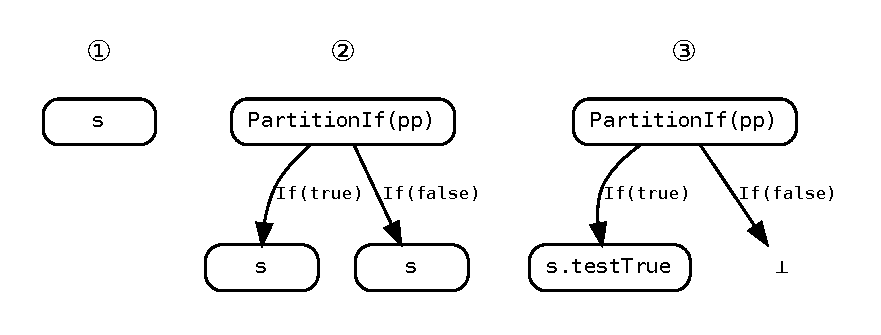
\includegraphics[]{Graphs/PartitionIf.pdf}
				\caption{The \code{PartitionIf} Directive}
				\label{figure:PartitionIf}
			\end{figure}

			Figure \ref{figure:PartitionIf} illustrates the basic transformations of the directive. Just before the analysis encounters the conditional statement, it will call the \code{before} method of the partitioned state containing a single leaf with some guest state \code{s}. The initial state in the figure is labeled with a \one. The state will then look up the directives stored in the \code{TracePartitioning} singleton and find the \code{PartitionIf} directive which it subsequently applies to the partitioning. This will result in a tree structure as depicted in \two. The node contains the directive and the left child represents the state following the \code{true} branch, as indicated by its token \code{If(true)}, while the right child represents the state following the \code{false} branch respectively. 

			During the further analysis, both branches will eventually be taken. When following the \code{true} branch, the \code{testTrue} method of the partitioned state will be called and will then be mapped to all the leaves of the partitioning. Subsequently, the state will inform all active directives that the \code{testTrue} method has been called and gives them a chance to change the partitioning. The \code{PartitionIf} directive makes use of that facility by setting the child representing the false branch to \code{Bottom}, representing the contradiction. The resulting state is depicted in \three.

			\begin{figure}
				\centering
				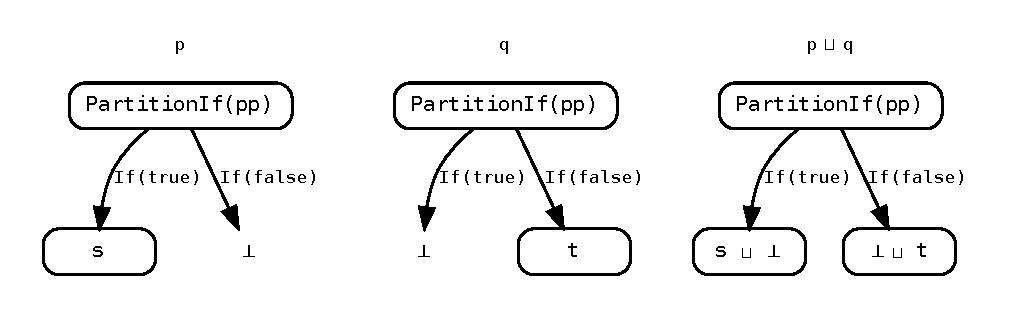
\includegraphics[width=\textwidth]{Graphs/PartitionIf_lub.pdf}
				\caption{Least Upper Bound on Join}
				\label{figure:PartitionIf::lub}
			\end{figure}

			In the subsequent analysis, the \code{false} branch remains effectively discarded until the two branches are joined together by taking the least upper bound over the over two complementary partitionings. This join operation is depicted in Figure \ref{figure:PartitionIf::lub}. The left state \code{p} is obtained after analyzing the \code{true} branch, the right state \code{q} after the \code{false} branch. Taking the least upper bound results in a new partitioning with the same directive where the least upper bound is applied to corresponding leaves of the tree.

		\end{subsection}

		% Merge

		\begin{subsection}{Merge}
			\label{subsection:Merge}

			The \code{Merge} directive differs from other directives in that it is the only one capable of reducing the size of the tree. It represents the inverse transformation of a given directive, stored in the \code{source} attribute. Upon application, the directive searches through the partitioning for nodes containing the generating directive and when it finds one, replaces it with the least upper bound of all its children.

			\begin{figure}[h]
				\centering
				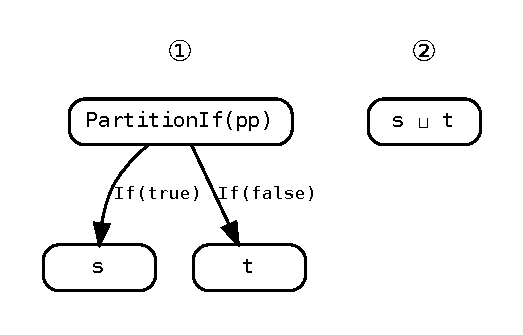
\includegraphics[]{Graphs/Merge.pdf}
				\caption{The \code{Merge} Directive}
				\label{figure:Merge}
			\end{figure}

			The application of the \code{Merge} directive for the \code{PartitionIf} from the previous section is depicted in Figure \ref{figure:Merge}.
		\end{subsection}

		% PartitionValue

		\begin{subsection}{PartitionValue}
			The next directive is called \code{PartitionValue}. Its purpose is to distinguish traces based on the value of a variable.

			\begin{figure}
				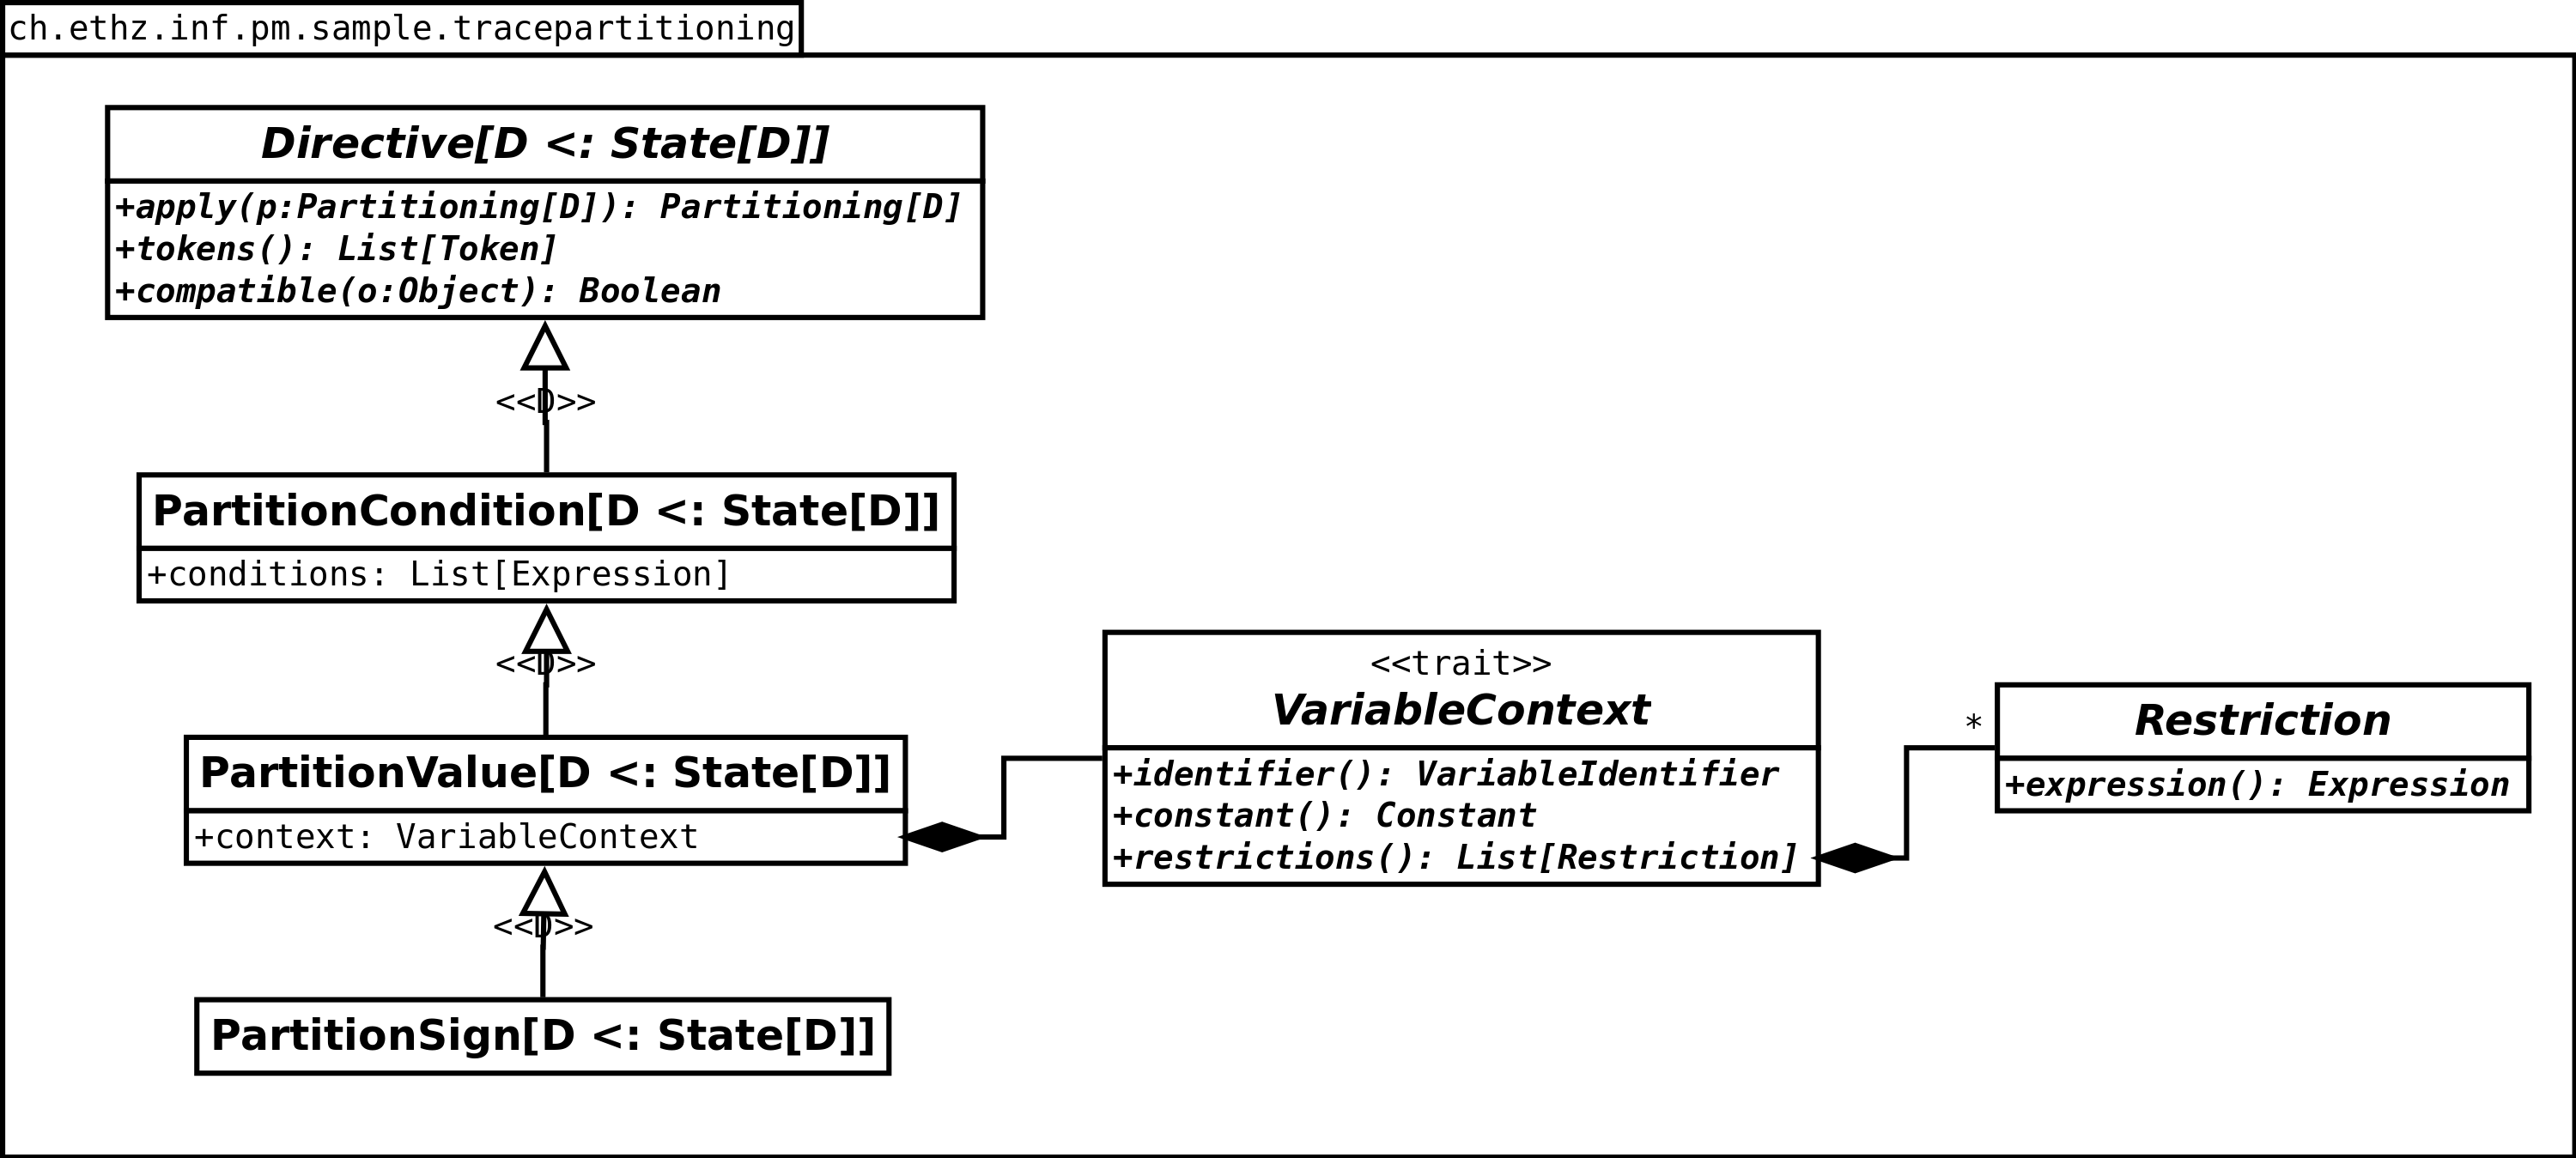
\includegraphics[width=\textwidth]{Diagrams/PartitionValue.png}
				\caption{\code{PartitionCondition} and \code{PartitionValue}}
				\label{figure:PartitionValueArchitecture}
			\end{figure}

			As Figure \ref{figure:PartitionValueArchitecture} shows, the implementation is based on the more general notion of a \code{PartitionCondition} directive. This directive creates a child assuming each condition it stores in form of a list of \code{Expression} objects.

			The \code{PartitionValue} directive imposes a restriction on what kind of conditions are supported. This restriction is represented by a \code{VariableContext} object that specifies which variable is restricted (\code{identifier}) and by what restrictions (\code{restrictions}). These restrictions are of type \code{Restriction} which is an abstract class generating an expression. The two implementing subclasses are \code{Value} and \code{Range}, representing, for some variable \code{x} and integers $i$ and $j$, expressions of the form \code{x == $i$} and \code{$j$ <= x \&\& x <= $i$} respectively. 

			\begin{figure}
				\centering
				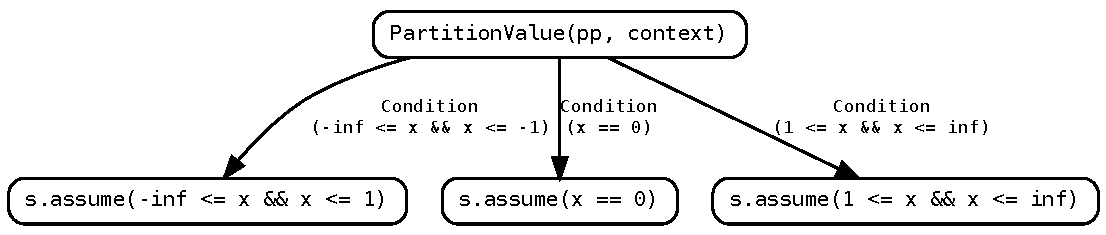
\includegraphics[width=\textwidth]{Graphs/PartitionValue.pdf}
				\caption{The \code{PartitionValue} Directive}
				\label{figure:PartitionValue}
			\end{figure}

			Functionally, there is no difference between the condition and value partitioning except that the latter simplifies the rather involved build up of the expressions.

			One more level of specialization is provided by the \code{PartitionSign} directive that splits an integer value into its three possible sign values.
		\end{subsection}

		% PartitionWhile

		\begin{subsection}{PartitionWhile}
			\label{section:PartitionWhile}

			The \code{PartitionWhile} is by far the most complex directive currently implemented. Unfortunately, its requirements pose some problems to the implementation using the current framework.

			\begin{figure}
				\centering
				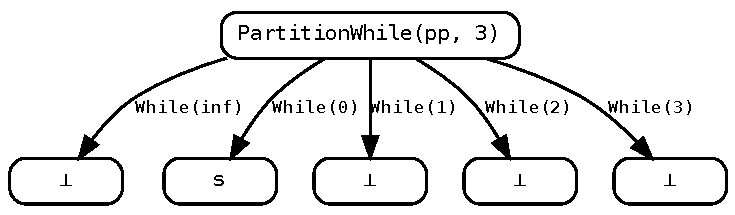
\includegraphics[]{Graphs/PartitionWhile.pdf}
				\caption{The \code{PartitionWhile} Directive}
				\label{figure:PartitionWhile}
			\end{figure}

			Figure \ref{figure:PartitionWhile} depicts the initial partitioned state after applying the directive. The directive takes two parameters. First, like all directives the program point, here pointing to the loop condition. The second parameter \code{n} denotes the number of times the loop is unrolled during the analysis. The resulting partitioned state has \code{n+2} children. The first child, identified by the \code{While(inf)} token, represents the executions that go through the loop more than \code{n} times. The second child with the token \code{While(0)} represents the traces that skip the loop completely. The rest of the states with the tokens \code{While(i)} collect the traces that iterate through the loop exactly \code{i} times.

			\begin{figure}
				\centering
				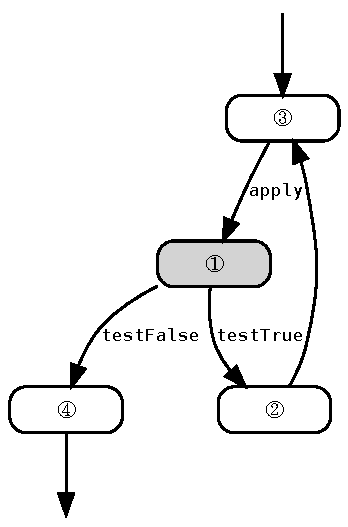
\includegraphics{Graphs/PartitionWhileControlFlow.pdf}
				\caption{Control Flow Graph for a Loop}
				\label{figure:PartitionWhileControlFlow}
			\end{figure}

			Maintaining these invariants during the analysis is quite tricky. Figure \ref{figure:PartitionWhileControlFlow} depicts the major stages involved in analyzing a loop. Here, \one represents the loop condition. Before evaluating the loop condition, the \code{PartitionWhile} directive is applied. When the condition is evaluated to true, the \code{testTrue} method is called and the analysis continues inside the loop at \two. The resulting state is then joined with the state coming from outside the loop at \three and the directive is once more applied to get back to the loop condition. The analysis continues by repeating the previously described steps or by following the \code{false} branch and leaving the loop structure by applying \code{testFalse} to \four.

			Starting with some initial state at \three and applying the directive initially results in the state depicted in Figure \ref{figure:PartitionWhile}. Note that applying the directive is required only once. When the partitioning already contains a \code{PartitionWhile} directive for the loop condition, it does not make sense to generate any further nodes. This is unlike, for example, the \code{PartitionIf} directive which, inside a loop and lacking a corresponding \code{Merge} directive, will split leaves with new nodes until the widening limit is reached.
			
			Entering the loop then calls \code{testTrue} on the state which in turn gives the directive the possibility to modify the partitioning. Having entered the loop means that the invariant for the \code{While(0)} child is being violated. This state will be analyzed in the loop and hence eventually exit the loop, making it effectively the child that should be mapped to by the \code{While(1)} token. Shifting the state one child to the right and marking the \code{While(0)} child with a contradiction restores the invariants for both leaves. The same shift to the right can restore the invariants for the rest of the \code{While(i)} states in future iterations. The \code{While(inf)} child needs some special attention. The shift of the \code{While(n)} will only wrap around if the state for \code{While(inf)} is \code{Bottom}. The other case happens when this shift has already happened and the state already represents the traces looping through more than \code{n} times. The former case is depicted in Figure \ref{figure:PartitionWhile::testTrue} and the code segment handling this piece of logic can be seen in Listing \ref{listing:PartitionWhile::testTrue}.

			\lstinputlisting[float=h, caption=The \code{testTrue} Method, label=listing:PartitionWhile::testTrue]{Source/PartitionWhile_testTrue.scala}

			\begin{figure}
				\centering
				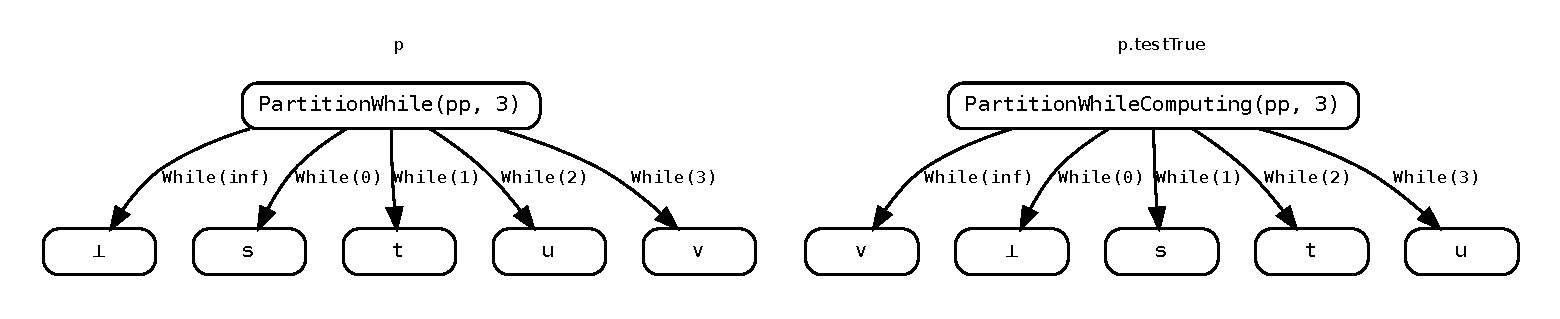
\includegraphics[width=\textwidth]{Graphs/PartitionWhile_testTrue.pdf}
				\caption{The Partitioned State Before and After \code{testTrue}}
				\label{figure:PartitionWhile::testTrue}
			\end{figure}

			Although, the handling of this directive is already a bit more complicated than, for example, the \code{PartitionIf} directive, the real trouble starts with the required non uniformity of the least upper bound operator. Consider the location \three in Figure \ref{figure:PartitionWhileControlFlow} from the perspective of a partitioned state coming from inside the loop \two. This state will be joined with a state that comes in two possible forms.

			\begin{enumerate}
				\item A state that also contains the \code{PartitionWhile} directive for the loop condition \one. This is the case if the loop in question itself is inside an other loop and the partitioned state is fed back.
				\item Some other state not containing the \code{PartitionWhile} directive for the condition at \one.
			\end{enumerate}

			The former case is handled just fine by the default implementation. The least upper bound will result in a new state where the leaves of the directive node are joined pairwise and since all the leaves satisfy the previously stated invariants, the resulting state will satisfy those as well. In the latter case however, this does not work. The other state represents traces that so far have not traversed the loop. Implicitly, this makes it the leaf of a \code{PartitionWhile} node for the token \code{While(0)} and it should be logically treated as such. 
			
			It is important to notice that this behavior is specific to the location \three in Figure \ref{figure:PartitionWhileControlFlow}. For states outside the loop, joining two states works as usual. This distinction between the partitioned state inside and outside the loop is addressed by two distinct directives representing either case. The reader may have already noticed in Figure \ref{figure:PartitionWhile::testTrue} that, aside from a shift of the leaves to the right, the directive also changes. The two directives are \code{PartitionWhile}, representing the general case outside the loop and \code{PartitionWhileComputing}, denoting the same directive inside the computation of the loop. As already hinted at, the former is transformed into the latter when entering the loop, that is when \code{testTrue} is called. The reverse happens when the loop is left with the application of the \code{testFalse} method.

			The distinction between the two cases is solely used in the lattice operations least upper bound, greatest lower bound and the widening. For all other intents and purposes they are equal. This fact is reflected by the \code{compatible} method. Moreover, the \code{PartitionWhile} directive is the reason why \code{compatible} was introduced in the first place instead of simply using the default \code{==} method.

			The \code{Directive} class has no way of influencing the least upper bound operation of two partitioned states and in my opinion has no business in doing so. However, as just demonstrated, the implementation of the \code{PartitionWhile} clearly requires to change the way joins operate. Assuming that this directive remains an exception\footnote{I can not think of any other possible directive with the same requirements}, it seems acceptable to have this little piece of logic removed from its natural setting.

			Listing \ref{listing:Node::lub} displays the final implementation of the least upper bound method of the \code{Node} class.

			\lstinputlisting[float=h, caption=The final \code{lub} Method in \code{Node}, label=listing:Node::lub]{Source/Node_lub.scala}

			The main differences compared with the simplified version from Listing \ref{listing:Node::lubSimplified} are the additional case distinctions for incompatible nodes. In case two nodes are joined and one of them contains a \code{PartitionWhileComputing} directive, instead of just returning \code{Top}, the join is computed as described above. When the argument is a leaf, the method checks whether the current node contains a \code{PartitionWhileComputing} directive and then performs the join accordingly.

		\end{subsection}
	\end{section}

	% USER INTERFACE

	\begin{section}{User Interface}
		\label{section:UserInterface}

		\sample comes with a small graphical user interface (GUI) that greatly simplifies running analyses. This section describes the main functionality of the user interface. I have made various changes both for improving usability in general and to be able to quickly generate directives used in the analysis. The application is written in \java and the interface was mostly created using \intellij's ``UI Designer'' plug-in.

		% Analysis Setup

		\begin{subsection}{Analysis Setup}
			Figure \ref{figure:GUI} shows a screenshot of the user interface as it is presented after running the application. 

			\begin{figure}
				\centering
				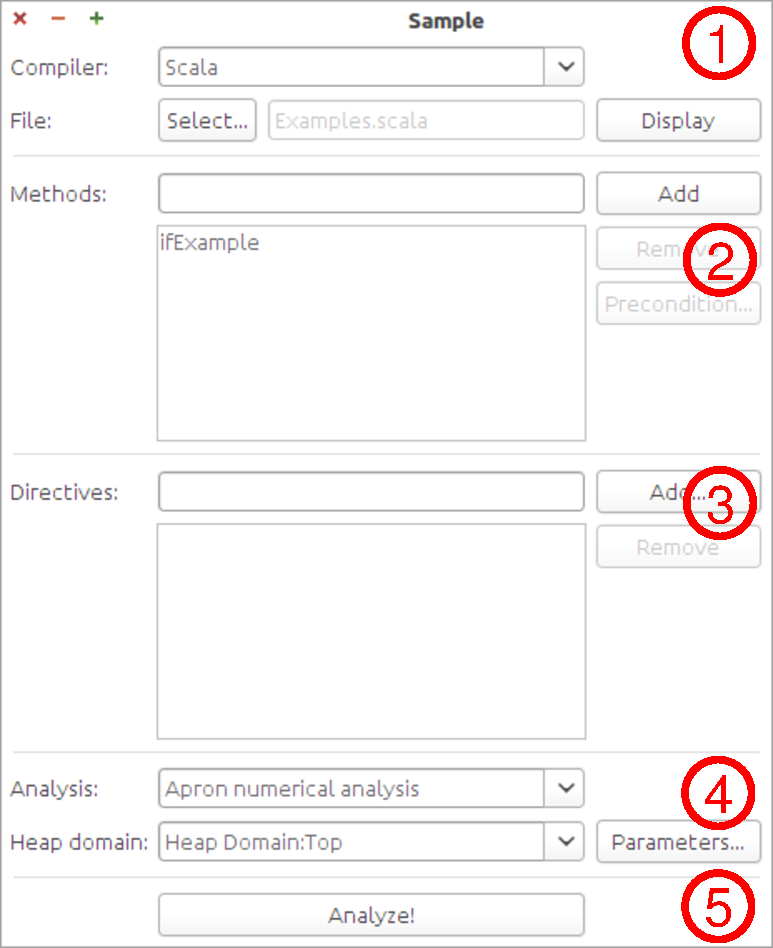
\includegraphics[scale=0.7]{Images/GUI.pdf}
				\caption{The Graphical User Interface}
				\label{figure:GUI}
			\end{figure}

			The user is asked in \one to first specify the compiler to use and to provide a source file to analyze. The chosen file can be displayed using the ``Display'' button to the right. The user can then edit a list of methods that should be analyzed in \two. Subsequently, a list of directives follows in \three. The directives can either be entered as a \code{String}, in which case the \code{Directive} companion object tries to parse the input, or by means of a wizard discussed later in this section. The next step in \four is to specify what kind of analysis to run. The choices here depend on the available plug-ins. Furthermore, a heap representation has to be picked. Once everything is set up, the ``Analyze'' button \five initiates the analysis.
		\end{subsection}

		% Adding Directives

		\begin{subsection}{Adding Directives}
			Pressing the ``Add'' button in the directives section starts the wizard. An example of a wizard helping to set up a \code{PartitionValue} directive is shown in \ref{figure:AddDirective}. 

			\begin{figure}
				\centering
				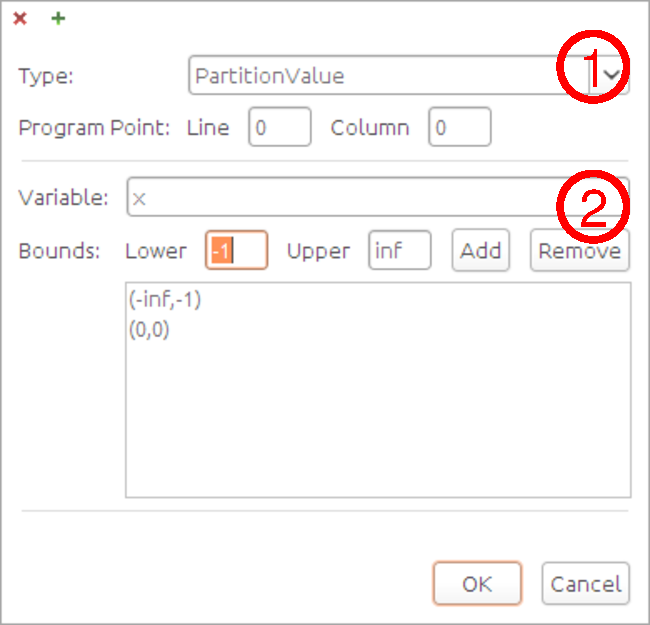
\includegraphics[scale=0.7]{Images/AddDirective.pdf}
				\caption{Adding a Directive}
				\label{figure:AddDirective}
			\end{figure}

			The top section, indicated by \one, of the wizard is common to all directives and consists of the choice of directive and an identifying program point. Choosing the right program point is currently a tedious task. However, displaying the source inside the user interface using the ``Display'' button and placing the cursor at the right location provides the line and column numbers in the lower left corner of the window.

			The rest of the panel, marked by \two, is directive specific. For the \code{PartitionIf} directive, no more parameters have to be specified. For \code{PartitionWhile} only the parameter \code{n} has to be set. The screenshot shows the additional parameters for \code{PartitionValue}. The variable over which to partition has to be chosen, here it is \code{x}. Furthermore, a list of intervals can be provided.
		\end{subsection}

		% Running the Analysis

		\begin{subsection}{Running the Analysis}
			Once the analysis is started, the interface might ask some further parameters before actually running the analysis. The \apron analysis, for example, provides a collection of several abstract domains, one of which has to be chosen. Furthermore, the property of interest for the analysis has to be selected. Again, the available choices are specific to the chosen analysis. For instance, the numerical domains provided by \apron all support the already mentioned \code{DivisionByZero} property that generates a warning for every possible division where the divisor can not be guaranteed to be non-zero.

			Once these parameters are set, the analysis can be run. Feedback is provided by a progress bar and some status updates. Once the analysis is terminated, a quick log is displayed to the user containing all generated output. This usually includes the warnings of the properties (or absence thereof) as well as some statistics about the analysis, for example, how much time has passed.

			\begin{figure}
				\centering
				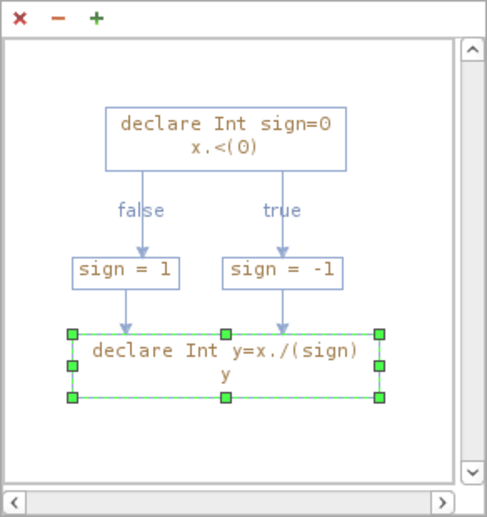
\includegraphics[scale=0.7]{Images/ShowGraph.pdf}
				\caption{The \code{ShowGraph} Property}
				\label{figure:ShowGraph}
			\end{figure}

			A special property supported by most analyses is the \code{ShowGraph} property. Unlike other properties it does not check any property during the analysis. Upon completion, it displays the control flow graph of the analyzed method. Figure \ref{figure:ShowGraph} shows such a control flow graph. The user can then click on the nodes to get a representation of the control flow graph execution, displaying the sequence of states of the block connected by the statements between them.
		\end{subsection}
	\end{section}

	% LIMITATIONS

	\begin{section}{Limitations}
		\label{section:Limitations}

		The current limitations of \sample naturally also apply to the trace partitioning implementation. This includes that calls to methods without contracts result in a total loss of information. Nonetheless, the implementation already includes some facilities to deal with different calling contexts. The \code{Void} token and its corresponding directive \code{PartitionNone}, for example, can be used to distinguish between different stacks in a state. Further information on the usefulness of this special construct can be found in \cite{mauborgne:rival05}.

		Furthermore, the limited availability of numerical types in \sample also limits the \code{PartitionValue} directive. However, the design of the directive has been made with multiple supported types in mind and the adaption, once more types become available, should not pose a problem.

		Generally, the implementation of most directives has been straightforward. I therefore consider the overall design to be quite flexible and hope it will prove easy to extend further. However, there are limitations which became apparent when implementing the \code{PartitionWhile} directive. Most of these have already been addressed in the previous section. The directive has an additional flaw which is unavoidable. While in general, the running time and convergence of the analysis with partitioned states depends heavily on how the directives and the widening limits are chosen, the \code{PartitionWhile} directive is problematic as soon as non-trivial loops, especially nested ones, are analyzed. This stems from the nature of the invariants imposed on the leaves. Changing the state of the leaf for \code{While(0)} affects all other leaves. Changing this one leaf invalidates all other leaves and the iteration computing the loop states has to reach a new fixed point. I speculate that an iteration algorithm aware of the partitioned states might provide some form of mitigation, though this subject is out of the scope of this thesis.
	\end{section}

\end{chapter}
